\documentclass[review]{elsarticle}

\usepackage{lineno,hyperref}
%\usepackage[utf8]{inputenc}
%\usepackage[english]{babel}
%\usepackage{authblk}
\usepackage{amssymb,amsmath,amsthm}
%\usepackage[pdftex]{graphicx}
%\usepackage{footnote}
%\usepackage{url}
%\usepackage{times,dsfont}
%\usepackage{fancyhdr}
%\usepackage{geometry}
%\pagestyle{fancy}
\modulolinenumbers[5]

\journal{Journal of \LaTeX\ Templates}

%%%%%%%%%%%%%%%%%%%%%%%
%% Elsevier bibliography styles
%%%%%%%%%%%%%%%%%%%%%%%
%% To change the style, put a % in front of the second line of the current style and
%% remove the % from the second line of the style you would like to use.
%%%%%%%%%%%%%%%%%%%%%%%

%% Numbered
%\bibliographystyle{model1-num-names}

%% Numbered without titles
%\bibliographystyle{model1a-num-names}

%% Harvard
%\bibliographystyle{model2-names.bst}\biboptions{authoryear}

%% Vancouver numbered
%\usepackage{numcompress}\bibliographystyle{model3-num-names}

%% Vancouver name/year
%\usepackage{numcompress}\bibliographystyle{model4-names}\biboptions{authoryear}

%% APA style
\bibliographystyle{model5-names}\biboptions{authoryear}

%% AMA style
%\usepackage{numcompress}\bibliographystyle{model6-num-names}

%% `Elsevier LaTeX' style
%\bibliographystyle{elsarticle-num}
%%%%%%%%%%%%%%%%%%%%%%%

\newcommand{\ts}{y}
\newcommand{\fullts}{{\bf \ts}}
\newcommand{\tspred}{\widehat{\ts}}
\newcommand{\stat}{f}
\newcommand{\statparam}{\theta_{predictor}}
\newcommand{\fullstat}{{\bf \stat}}
\newcommand{\lag}{h}
\newcommand{\window}{w}
\newcommand{\tswindow}{{\bf \ts}}
\newcommand{\meants}{\Bar{\ts}}
\newcommand{\rnnwindow}{{\bf \rnninput}}
\newcommand{\rnninput}{z}
\newcommand{\rnn}{\textsc{rnn}}
\newcommand{\rnnparam}{\theta_{corrector}}
\newcommand{\err}{err}
\newcommand{\errwindow}{{\bf \err}}
\newcommand{\rnnmodel}{\textsc{rnn}}
\newcommand{\ws}{w}
\newcommand{\fullws}{{\bf \ws}}
\newcommand{\wswindow}{{\bf \ws}}
\newcommand{\concatinput}{x}
\newcommand{\fullconcatinput}{{ \bf \concatinput}}
\newcommand{\numberts}{10000}
\newcommand{\threshold}{\eta}
\newcommand{\predictor}{\mathrm{RNN}_p}
\newcommand{\classifier}{\mathrm{RNN}_c}
\newcommand{\remainder}{r}
\newcommand{\hiddenregime}{U}


\begin{document}

\begin{frontmatter}

\title{HERMES: Hybrid Error-corrector Model with inclusion of External Signals for nonstationary fashion time series}
%\tnotetext[mytitlenote]{Fully documented templates are available in the elsarticle package on \href{http://www.ctan.org/tex-archive/macros/latex/contrib/elsarticle}{CTAN}.}

%% Group authors per affiliation:
\author[mymainaddress,mysecondaryaddress]{Etienne DAVID}

%% or include affiliations in footnotes:
\author[mysecondaryaddress]{Jean BELLOT}

\author[mymainaddress]{Sylvain LE CORFF} 

\address[mymainaddress]{\small  Samovar, T\'el\'ecom SudParis,  D\'epartement CITI, Institut Polytechnique de Paris, France.}
\address[mysecondaryaddress]{Heuritech, 71 Rue Réaumur, 75002 Paris, France.}

\begin{abstract}
Developing models and algorithms to draw causal inference for time series is a long standing statistical problem. It is crucial for many applications, in particular for fashion or retail industries, to make optimal inventory decisions and avoid massive wastes. By tracking thousands of fashion trends on social media with state-of-the-art computer vision approaches, we propose a new model for fashion time series forecasting. Our contribution is  twofold. We first provide publicly\footnote[1]{\url{http://files.heuritech.com/raw_files/f1_fashion_dataset.tar.xz}} the first fashion dataset gathering \numberts\ weekly fashion time series. As influence dynamics are the key of emerging trend detection, we associate with each time series an external weak signal representing behaviors of influencers. Secondly, to leverage such a complex and rich dataset, we propose a new hybrid forecasting model. Our approach combines per-time-series parametric models with seasonal components and a global recurrent neural network to include sporadic external signals. This hybrid model provides state-of-the-art results on the proposed fashion dataset, on the weekly time series of the M4 competition \cite{makridakis2018m4}, and illustrates the benefit of the contribution of external weak signals.
\end{abstract}

\begin{keyword}
Hybrid models, Recurrent neural networks, Time series.
\end{keyword}

\end{frontmatter}

\linenumbers

\section{Introduction}
\label{sec:introduction}


Multivariate time series forecasting is a widespread statistical problem with  many applications, see for instance \cite{sarkka2013bayesian, douc2014nonlinear, zucchini2017hidden} and the numerous references therein.
 %Due to the diversity of applications and use cases, a multitude of models have been proposed. 
Parametric generative models provide explainable predictions with statistical guarantees based on a precise modeling of the predictive distributions of new data based on a record of past observations. %The parameters of these models are usually estimated using a sequence of observations of the target time series. 
Calibrating these models, for instance using maximum likelihood inference, often requires a fair amount of tuning to design a time series-specific model to provide  accurate forecasts and sharp confidence intervals.  Depending on the use case, statistical properties of the signal and the available data, many families of models have been proposed for time series.  The exponential smoothing model \cite{RePEc:inm:oropre:v:9:y:1961:i:5:p:673-685}, the Trigonometric Box-Cox transform, ARMA errors, Trend, and Seasonal components model (TBATS) \cite{doi:10.1198/jasa.2011.tm09771}, or the ARIMA with the Box-Jenkins approach \cite{box2015time} are for instance very popular parametric generative models.  Hidden Markov models (HMM) are also widespread and presuppose that available observations are defined using missing data describing the dynamical system. This hidden state is assumed to be a Markov chain such that at each time step the received observation is a random function of the corresponding latent data.  Although hidden states are modeled as a Markov chain, the observations arising therefrom have a complex statistical structure. %Introducing latent hidden states, they assume that the predictive distribution is not unique and constant in time but multiple and lead by the values of the hidden states changing during time. 
In various applications where signals exhibit non-stationarities such as trends and seasonality, classical HMM are not adapted. However, \cite{touron2017modeling}  recently proposed seasonal HMM, assuming that transition probabilities between the states, as well as the emission distributions, are not constant in time but evolve in a periodic manner. Strong consistency results were established in \cite{touron2019consistency} and Expectation Maximization based numerical experiments were proposed.
Although these works provide promising results, HMM are computationally expensive to train and are not yet well studied for seasonal  sequences with thousands of components.
 
In many fields, single or few time series have become thousands of sequences with various statistical properties. In this new context, classical time series specific statistical models show limitations when dealing with numerous heterogeneous data. Recurrent neural networks and recent sequence to sequence deep learning architectures offer very appealing numerical alternatives thanks to their capability of leveraging any kind of heterogeneous multivariate data, see for instance \cite{ hochreiter1997long,vaswani2017attention, 8614252, li2019enhancing, lim2019temporal,salinas2020deepar}. The DeepAR model proposed in \cite{salinas2020deepar} provides a global model from many time series based on a multi-layer recurrent neural network with LSTM cells. More recently, applications using the Transformer model have been proposed  \cite{li2019enhancing}. The Temporal Fusion Transformers (TFT) approach is a direct alternative to the DeepAR model \cite{lim2019temporal}.  Unfortunately, all these solutions suffer from two main weaknesses. Firstly, many of them are black-boxes  as the final forecast usually does not come with a statistical guarantee  although a few recent works focused on measuring uncertainty in recurrent neural networks, see  \cite{martin2020monte}. Secondly, without a fine preprocessing and well chosen hyper-parameters, these methods may lead to poor results and be outperformed by traditional statistical models, see \cite{makridakis2018m4}.

In this paper, we consider a  new time series forecasting application referred to as {\em fashion trends prediction}. Based on a cutting-edge image recognition technology, we built the first fashion dataset containing \numberts\ weekly sequences  of fashion trends on social media  from 01-01-2015 to 01-01-2019. This dataset has very appealing properties:  all time series have the same length, no missing value and there is no sparse time series even for niche trends. The originality of our dataset comes from the fact that additional external weak signals can also be introduced. With our fashion expertise, we detected several groups of highly influential fashion users. Analyzing their specific behaviours on social media, we associate with each time series an external weak signal representing the same fashion trends on a sub-category of users. They are called weak signals because they are often alerts or events that are too sparse, or too incomplete to allow on their own an accurate estimation of their impact on the prediction of the target signal. With this totally new application, we aim at designing a model able to deal with such a large dataset, leveraging  complex external weak signals and finally providing the most accurate forecasts.
 
Recurrent neural networks are appealing to tackle our forecasting problem due to their capability of leveraging external data.  Recently, hybrid models combining deep neural network (DNN) architectures with widespread statistical models to deal with seasonality and trends have been proposed, see for instance  \cite{zhang2003time,jianwei2019novel,bandara2020lstm}. The approach providing the most striking results was proposed in  \cite{smyl2020hybrid} in the context of the M4 forecasting competition \cite{makridakis2020m4}.  Given a large dataset, a per-time-series multiplicative exponential smoothing model was introduced to estimate simple but fundamental components for each time series and compute a first prediction. Then a global recurrent neural network was trained on the entire dataset to correct errors of the previous exponential smoothing models. 

Following this work, we present in this paper HERMES, a new hybrid recurrent model for time series forecasting with inclusion of external signals. This new architecture is decomposed  into two parts: local predictors and a global corrector.  First, a per-time-series parametric statistical model is trained on each sequence. Then, a global recurrent neural network is trained to evaluate and correct the forecast weaknesses of the first collection of models. The external weak signals reveal the real potential of the hybrid approach: a global neural network, able to leverage large amounts of heterogeneous data, deal with any kind of external weak signals, learn context and finally correct weaknesses and errors of parametric models.

The paper is organized as follows. Section~\ref{sec:hybrid} introduces the proposed hybrid model. Then, the new fashion dataset provided with this article is presented in Section~\ref{sec:dataset}. Section~\ref{sec:exp} describes the HERMES results and comparisons with several benchmarks. Finally, a general conclusion and some research perspectives are given in  Section~\ref{sec:conclusion}.

\section{Hybrid model with external signals}
\label{sec:hybrid}
We introduce a new hybrid approach for time series forecasting  composed of two parts: a collection of per-time-series parametric models, and a global error-corrector neural network train on all time series. Per-time-series parametric models are used to learn local behaviours, to normalize sequences by removing trends and seasonality,  and to compute a first forecast. Then, gathering information of the first predictions and external variables, a recurrent neural network is trained to correct the predictions provided by the first collection of per-time-series models.

Consider $N\geqslant 1$ time series. For all $1\leqslant n \leqslant N$ and $1\leqslant t \leqslant T$, let $\ts_t^n$ be the value of the $n$-th sequence at time $t$ and  $\fullts^n = \{\ts_t^n\}_{1\leqslant t \leqslant T}$ be all the values of this sequence. The objective of this paper is to propose a model to  forecast all time series in a given time frame  $\lag \in \mathbb{N}$, i.e. we aim at sampling $\{\ts^n_{T+1:T+\lag}\}_{1\leqslant n \leqslant N}$ based on $\{\ts^n_{1:T}\}_{1\leqslant n \leqslant N}$.


\subsection{Per-time-series predictors}
The time-series-specific predictors compute, for each sequence, a first $\lag$-ahead prediction based on the past. For all $1\leqslant n \leqslant N$, we note $\stat^n(.;\statparam^n)$ the $n$-th parametric model of the $n$-th sequence where $\statparam^n$ are  unknown parameters. Given the sequences $\{\ts^n_{1:T}\}_{1\leqslant n \leqslant N}$ and the estimated  parameters $\{\statparam^n\}_{1\leqslant n \leqslant N}$, the time-series-specific forecasts $\{\tspred^{pred,n}_{T+1:T+\lag|T}\}_{1\leqslant n \leqslant N}$ are, for all $n \in \{1,\ldots,N\}$, for all $i \in \{1,\ldots,\lag\}$,
$$
\tspred^{pred,n}_{T+i|T} = \stat^n(\ts^n_{1:T};\statparam^n)_i\,.
$$
During the M4 competition, the hybrid model of \cite{smyl2020hybrid} was based on a multiplicative exponential smoothing model as the time-series-specific predictor. However, on sporadic time series, this choice leads to poor results and instability. In this paper, a more general framework able to deal with any kind of per-time-series models is provided. In Section~\ref{sec:exp}, two versions of our framework are proposed. The first one is based on an  exponential smoothing as a reference similar to the baseline \cite{smyl2020hybrid} and the second one uses a TBATS model \cite{doi:10.1198/jasa.2011.tm09771} which provides better results as this parametric model includes  Fourier representations with time varying coefficients, and ARMA error correction. 

In the specific application of fashion trends prediction, two main forms of standard weaknesses were detected and defined for univariate parametric forecasts. The first one is a weakness of definition, when the model is not well defined for its forecasting task. For instance, an additive model provides good predictions on time series with additive seasonality but fails at handling multiplicative seasonalities. The second form, harder to detect and correct, is the weakness of information. For non stationary time series, huge changes of behaviours are not always predictable using the past of the sequence. In somes cases, these changes depend on external variables not considered by univariate parametric models. The difficulty is that the exact influence of external variables on the main signal is mostly unknown. This motivates the introduction of a global RNN trained on all time series and able to consider and leverage external signals. First forecast example of our new hybrid model is given in Figure~\ref{fig:introexamples}.


\begin{figure*}
\centering
%\begin{subfigure}{1.\textwidth}
 % \centering
  %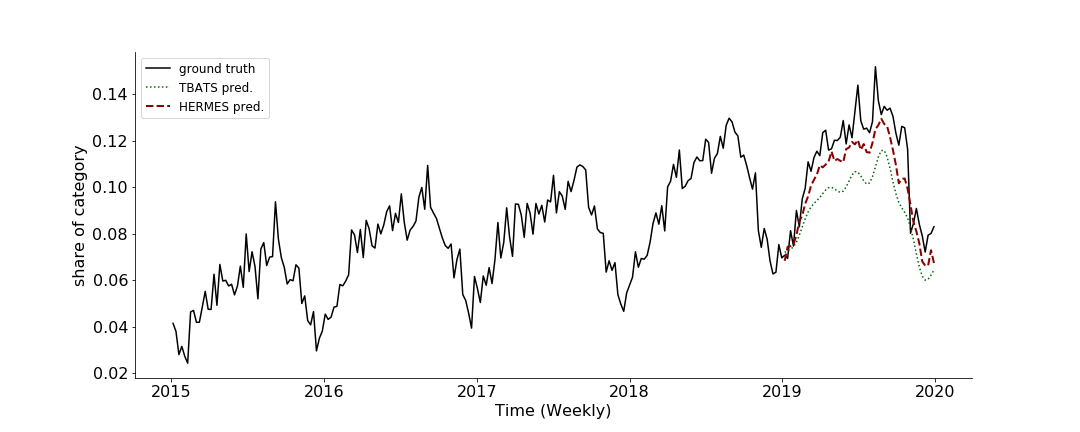
\includegraphics[width=\linewidth]{figure/us_female_shoes}
  %\caption{Time series representing a shoes fashion trend for female in The United States.}
 % \label{fig:introexamples:sub1}
%\end{subfigure}
%\begin{subfigure}{1.\textwidth}
  %\centering
  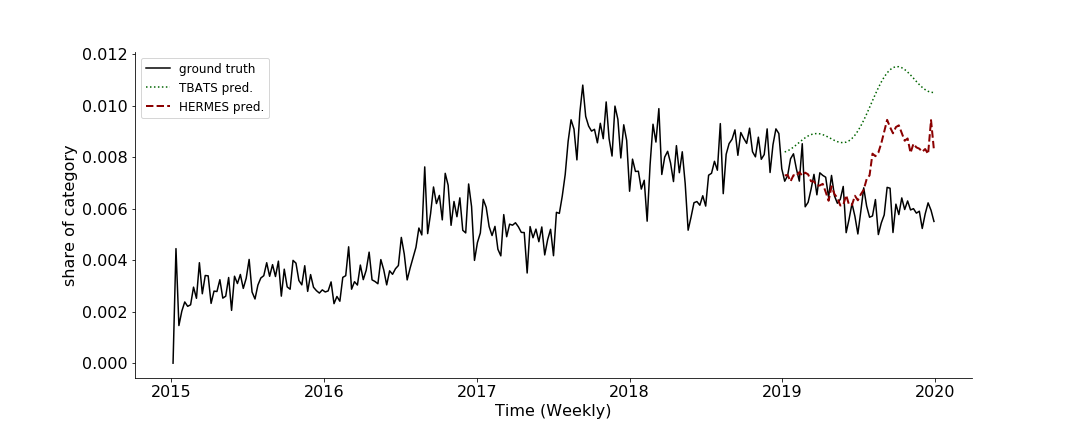
\includegraphics[width=\linewidth]{figure/br_female_texture_verticalstripe}
 % \caption{Time series representing the vertical stipes texture fashion trend for female in Brazil.}
  %\label{fig:introexamples:sub2}
%\end{subfigure}
\caption{Hermes forecast examples. In green the prediction of the TBATS per-time-series predictors. In red the final forecast of our HERMES hybrid model.  Time series representing the vertical stipes texture fashion trend for females in Brazil.}%(Top) Time series representing a shoes fashion trend for females in The United States. (Bottom) Time series representing the vertical stipes texture fashion trend for females in Brazil.}
\label{fig:introexamples}
\end{figure*}

\subsection{Error-corrector recurrent model}

The second part of the model is a global RNN, trained on all the $N$ sequences to correct the weaknesses of the first per-time-series parametric models. This task requires a thorough data pre-processing as recurrent neural networks training is highly sensitive to the scale of the data and requires well-designed inputs. Since no assumption about the scale of our time series was made, inputs require a careful normalization before being fed to the RNN.


Let $\window \in \mathbb{N}$ be the window size, usually this window is proportional to the forecast horizon $\window \propto \lag$. The RNN input is defined as the following  normalized, deseasonalized and rescaled sequence $\rnnwindow^n_T = \{\rnninput^{n}_{T-\window+i|T}\}_{1\leqslant i \leqslant w}$, where, for all $1\leqslant n \leqslant N$, $1\leqslant i \leqslant w$ and $k = i - h\lfloor i/h \rfloor$, 
$$
\rnninput^{n,T}_{T-w+i|T} = \frac{\ts^n_{T-w+i} -\tspred^{pred,n}_{T+k|T}}{\meants^n_T}\,,\quad \meants^n_T = \frac{1}{w}\sum_{i = 1}^{w}\ts^n_{T-w+i}\,.
$$
Let $\rnn(.;\rnnparam)$ be the recurrent neural network model where $\rnnparam$ are  unknown parameters. Given the RNN input sequences $\{\rnnwindow^n_T\}_{1\leqslant n \leqslant N}$ and the global RNN estimated parameters $\rnnparam$, the error-corrector predictions $\{\tspred^{corr,n}_{T+1:T+\lag|T}\}_{1\leqslant n \leqslant N}$ are, for all $n \in \{1,\ldots,N\}$, for all $i \in \{1,\ldots,\lag\}$,
$$
\tspred^{corr,n}_{T+i|T} = \rnn(\rnnwindow^n_T;\rnnparam)_i \cdot \meants^n_T\ \,.
$$
Our hybrid model forecast is, for all $1\leqslant n \leqslant N$ and all $i \in \{1,\ldots,\lag\}$,
\begin{align}
\label{eq:nows:full:model}
\tspred^n_{T+i|T}  &= \tspred^{pred,n}_{T+i|T} +  \tspred^{corr,n}_{T+i|T} \\
&= \stat^n(\ts^n_{1:T};\statparam^n)_i +  \rnn(\rnnwindow^n_T;\rnnparam)_i \cdot \meants^n_T\,.\nonumber
\end{align}


\subsection{Weak signal}

Using well-fitted time-series-specific parametric models, the new hybrid network corrects the first form of weakness and provides very good performance on the fashion dataset, see Table~\ref{tab:metricresults}. Then, to correct the second form of weakness, in addition to the $N$ target time series, $K \times N$ external sequences indexed from $0$ to $T$ are considered. For all $1\leqslant n \leqslant N$, $1\leqslant k \leqslant K$ and  $1\leqslant t \leqslant T$, let $\ws^{n,k}_t$ be the value of the $k$-th external sequence at time $t$ associated with the sequence $\fullts^n$. Let  $\fullws^n = \{\{\ws_t^{n,k}\}_{1\leqslant t \leqslant T}\}_{1\leqslant k \leqslant K}$ be all the values of the weak signals associated with the $n$-th sequence. In addition, let $\fullws^n_T = \{\{\ws_{T-w+i}^{n,k}\}_{1\leqslant i \leqslant \window}\}_{1\leqslant k \leqslant K}$ be only the last $\window$ terms of the sequence. Concatenating $ \rnnwindow^n_T$ and $\fullws^n_T$, a new input for the RNN is defined:   
\begin{align*}
\fullconcatinput^n_T &= \{\concatinput^n_{T-w+i|T}\}_{1\leqslant i \leqslant w}\\
&= \{\rnninput^n_{T-w+i|T}, \ws^{n,1}_{T-w+i},...,\ws^{n,K}_{T-w+i}\}_{1\leqslant i \leqslant w}\,.
\end{align*}
Finally, for all $1\leqslant n \leqslant N$ and for all $i \in \{1,\ldots,\lag\}$ the final prediction becomes:
%$$
%\tspred^n_{T+i|T} 
%= \etspred^{ets,n}_{T+i|T} +  \rnnmodel(\fullconcatinput^n_T)_{T+i} \times \meants^n_T
%$$
\begin{align}
\label{eq:withws:full:model}
\tspred^n_{T+i|T}  &= \tspred^{pred,n}_{T+i|T} +  \tspred^{corr,n}_{T+i|T}\\
& = \stat^n(\ts^n_{1:T};\statparam^n)_i +  \rnn(\fullconcatinput^n_T;\rnnparam)_i \cdot \meants^n_T\,.\nonumber
\end{align}
An illustration of the proposed  model is displayed in Figure~\ref{fig:architecture}.

\begin{figure}
  \centering
    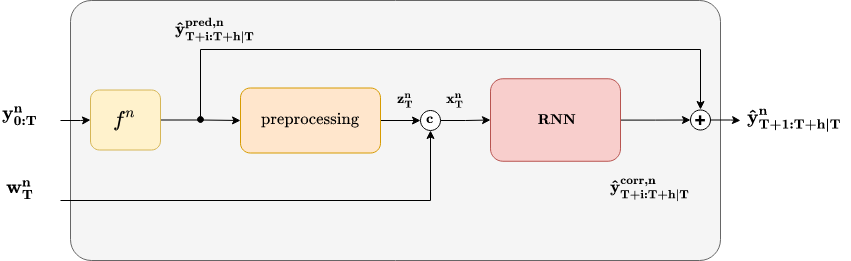
\includegraphics[width=1\linewidth]{figure/HERMES_archi.png}
  \caption{Architecture of the hybrid model with weak signals.}
\label{fig:architecture}
\end{figure}


\section{Fashion dataset with external weak signals}
\label{sec:dataset}

\subsection{Translate fashion to data}
\label{sec:dataset:a}
A collection of vision neural networks were designed and trained  at detecting clothes details on pictures: type of clothing (pants, shoes, tops, etc.), form, size, color, texture, etc. Then, fashion experts designed fashion trends by aggregating these clothes details: a meaningful combination of items that represent an existing trend in the fashion sphere. To finely represent human behaviours based on social media, a group of thousands of random users, called a panel, was created on several geolocalisations. Analyzing every day images shared on social networks by these panels with our computer vision algorithms, we can translate the history of thousands of fashion trends in thousands of time series.  All sequences have 261 time steps, from 2015-01-05 to 2019-12-31 with weekly values and no missing values. Each value represents the number of users posts in a week where computer vision algorithms detected the fashion trend.  As an illustration, an example of fashion time series is given in Figure~\ref{fig:normalization}.

\subsection{Fashion dataset}
\label{sec:dataset:b}

Due to the increasing use of social media and behaviour changes, a normalization step is applied to the raw sequences. Each fashion trend is divided by its hierarchical parent category trend. Moreover, in order to avoid removing the seasonality of all sequences, we deseasonalized the hierarchical parent category trend before the normalization. For instance, as displayed in Figure~\ref{fig:normalization}, the raw Jersey Top trend for females in China is divided by the deseasonalized global Top trend for females in China. The final normalized sequence is expressed in share of category.

We therefore introduce a new dataset for fashion time series forecasting.  It contains a sample of $\numberts$ anonymized and  normalized fashion trends for men and women, in 9 different categories and 5 geozones. An overview of it can be found in Table~\ref{tab:fashiondataset}. This collection of $\numberts$ fashion trends was selected in order to represent finely the issues faced by the fashion industry. For instance, some sequences show complex behaviours with sudden changes, referred to as emerging or declining trends. A central point of this work is to accurately detect and forecast such trends.

\begin{figure*}
\centering
%\begin{subfigure}{1.\textwidth}
 % \centering
  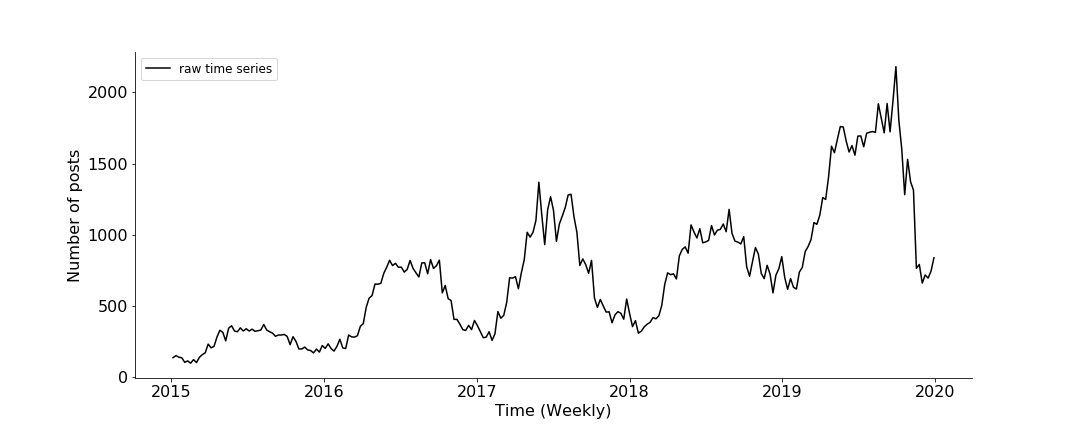
\includegraphics[width=1.\linewidth]{figure/cn_female_top_raw}
%  \caption{Time series representing the raw signal of a top fashion trend for female in China}
 % \label{fig:normalization:sub1}
%\end{subfigure}
%\begin{subfigure}{1.\textwidth}
 % \centering
  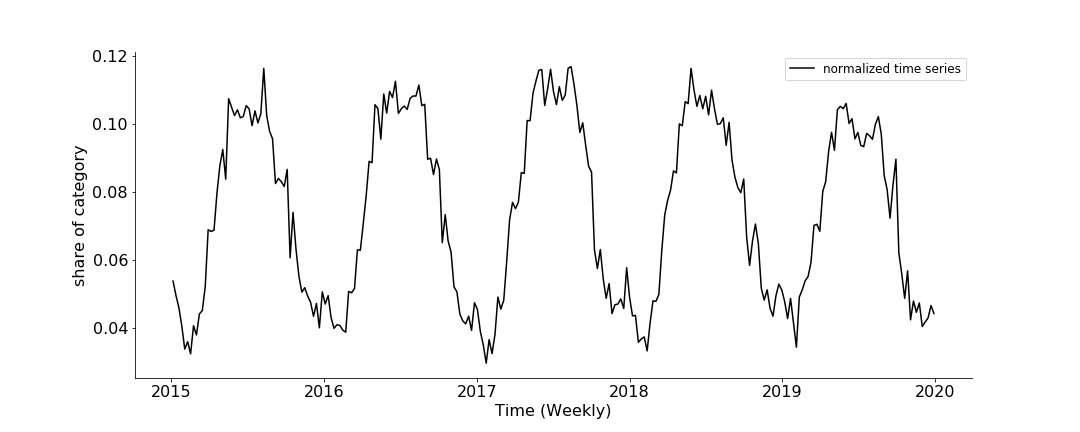
\includegraphics[width=1.\linewidth]{figure/cn_female_top_norm}
  %\caption{Time series representing the normalized signal of a top fashion trend for female in China.}
  %\label{fig:normalization:sub2}
%\end{subfigure}
\caption{Example of difference between the raw sequence and the normalized one. In this example, we normalize by the deseasonalized global top fashion trend for females in China. (Top) Time series representing the raw signal of a top fashion trend for females in China. (Bottom) Time series representing the normalized signal of a top fashion trend for females in China.}
\label{fig:normalization}
\end{figure*}

\begin{table*}
  \caption{Fashion time series overview. For each couple geozone/category, the table gives the number of trends (Female/Male).}
\label{tab:fashiondataset}
  \centering
  \resizebox{0.65\width}{!}{
  \begin{tabular}{l||lllllllll}
    %hline
    \\
    &  \textbf{Top}  & \textbf{Pants} & \textbf{Short} & \textbf{Skirt} & \textbf{Dress} & \textbf{Coat} & \textbf{Shoes} & \textbf{Color} & \textbf{Texture}  \\
    \hline
    \hline
    \\
\textbf{United States} & 411/208 & 149/112 & 47/22 & 29/- & 20/- & 208/151 & 293/86 & 38/44 & 85/81\\
     \textbf{Europe} & 409/228 &  134/114 & 48/21 & 28/- & 20/- & 211/159 & 303/78 & 41/42 & 87/74\\
     \textbf{Japan} &  403/218 & 136/107 & 49/31 & 28/- &  23/- & 185/149 &  311/78 & 46/42 &  92/65\\
     \textbf{China} &  424/202 & 147/114 & 46/29 & 27/- &  27/- & 178/161 &  310/78 & 41/47 &  88/77\\
     \textbf{Brazil} &  431/222 & 134/117 & 49/27 & 30/- &  28/- & 203/152 & 311/76 & 48/41 & 107/84\\
     \\
     %\hline
     \textbf{Total} & 2078/1078 & 700/564 & 239/130 & 142/- & 118/- & 985/772 & 1528/396 & 214/216 & 459/381\\
    %\hline
  \end{tabular}
  }
\end{table*}

\subsection{Weak signal}

In theoretical fashion dynamics \cite{rogersdiffusion}, different categories of adopters follow a trend in succession, resulting in several adoption waves. %In this way, a weak signal for each sequence is added to the proposed dataset.
Numerous social media influencers were selectioned by hand by fashion experts. By aggregating them, a specific ``fashion-oriented`` panel is created. With the same methodology as for the main panel described in Section~\ref{sec:dataset:a} and Section~\ref{sec:dataset:b}, a normalized time series representing each fashion trend on this specific population is created. We named \textit{fashion-forwards} this weak signal.  For all trends $\{y_t\}_{1\leqslant t\leqslant T}$, let $\ts_t^{f,n}$ be the value of the $n$-th \textit{fashion-forwards} sequence at time $t$ and  $\fullts^{f,n} = \{\ts_t^{f,n}\}_{1\leqslant t \leqslant T}$ be all the values of this sequence.
As we want to detect shifts between the main signal and the fashion forward signal, the following input is computed for our hybrid model:  for all $n \in \{1,\ldots,N\}$, for all $t \in \{1,\ldots,T\}$,
$$
\ws^{f,n}_{t} = \frac{\ts_t^{f,n}}{\ts_t^{f,n}+\ts_t^{n}}\,.
$$
Values close to 0.5 indicate a similar behaviour between the influencers panel and the general panel. For instance, an impressive emerging fashion shoes trend with its \textit{fashion-forwards} weak signal is represented in Figure~\ref{fig:oneemergingtrend}. 


%Secondly, depending of the number of followers, the general panel of users is divided in three sub-groups: users with less than 1350 followers, users with a number of followers between 1350 and 7000 and users with more than 7000 followers. Repeating the previous methodology on each sub-panel, three normalized time series for each time series are created.  Again, the motivation here is to detect behaviour gaps between different parts of the society that could lead to changes in the main signal. Let $\ts_t^{\ell,n}$,$\ts_t^{m,n}$ and $\ts_t^{h,n}$ be the value of the $n$-th \textit{followers-low},\textit{followers-mid} and \textit{followers-high} sequence at time $t$ and  $\fullts^{\ell,n} = \{\ts_t^{f,n}\}_{1\leqslant t \leqslant T}$, $\fullts^{m,n} = \{\ts_t^{f,n}\}_{1\leqslant t \leqslant T}$, $\fullts^{h,n} = \{\ts_t^{f,n}\}_{1\leqslant t \leqslant T}$ be all the values of these sequences. Two inputs for our hybrid model are computed: for all $n \in \{1,\ldots,N\}$, for all $t \in \{1,\ldots,T\}$,
%\begin{align*}
%\ws^{\ell,n}_{t} = \frac{\ts_t^{\ell,n}}{\ts_t^{\ell,n}+\ts_t^{m,n}+\ts_t^{h,n}}\,,\quad \ws^{h,n}_{t} = \frac{\ts_t^{h,n}}{\ts_t^{\ell,n}+\ts_t^{m,n}+\ts_t^{h,n}}
%\end{align*}  
%values close to 0.3 indicate a similar behaviour between the three sub-panels and the general panel.
%
%In addition to the fashion dataset, for each time series, the three weak signals $\ws^{f}$,$\ws^{\ell}$ and $\ws^{h}$ are added. They are frequently sparse for micro trends and they often lack interest in common fashion trends. However, in several examples, they are fundamental to detect the future fashion evolutions, as illustrated in Section~\ref{sec:exp}. 


\begin{figure*}
  \centering
    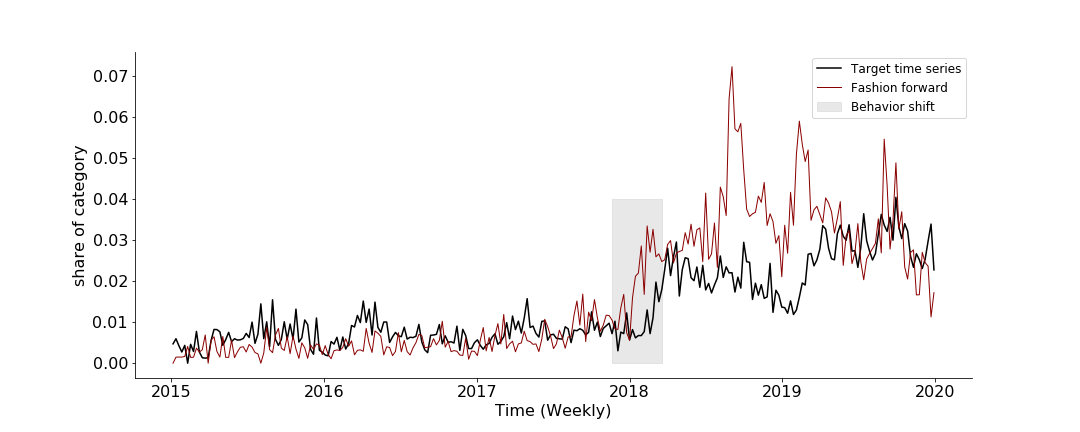
\includegraphics[width=1.\linewidth]{figure/ff_example}
  \caption{A shoes trend of the fashion dataset. In black the main signal and in red its associated \textit{fashion-forward} weak signal. The shift between these two signals at the end of 2017/beginning of 2018 announces the future burst of the trend.}
\label{fig:oneemergingtrend}
\end{figure*}





\section{Experimental results}
\label{sec:exp}

\subsection{Training}
The dataset is split into three blocks, {\em train}, {\em eval} and {\em test} sets. The 3 first years are used as the {\em train} set, the 4th year is kept for the {\em eval} set and the {\em test} set is made of the last year. The hybrid model is trained to compute a one-year ahead prediction, $\lag$ equal to 52, and the window size $\window$ is fixed at 104.
Using the two first years of the {\em train} set, a first per-time-series parametric model for each time series is fitted. With the resulting collection of local models, a forecast of the third year is computed for each sequence. Corrector inputs are finally computed and the RNN is trained at correcting this first collection of third-year forecasts. For the {\em eval} set, per-time-series predictors are fitted a second time using the three first years and forecasts of the fourth year are computed. The {\em eval} set is used during  training to control the learning of the RNN model and prevent overfitting. The per-time-series predictors are fitted a last time for the {\em test} set using the four first years. The final accuracy measures of all our models are computed on this {\em test} set. As an illustration, an example of our split is shown in Figure~\ref{fig:train_eval_test_set}.

For the first parametric per-time-series models, existing Python or R libraries are used to estimate the different parameters $\statparam^n$.  Depending of the choice of local parametric models, two versions of HERMES are proposed. The first one uses as predictors an additive exponential smoothing model as a reference close to \cite{smyl2020hybrid}. The second one uses the TBATS model of \cite{doi:10.1198/jasa.2011.tm09771} and  achieves the best accuracy results on the fashion dataset. The neural network architecture is summarized in Figure~\ref{fig:rnn_architecture}. It is composed of 3 LSTM layers of shape 50 and a final Dense layer to provide the correct output dimension. A classical Adam optimizer is used with a learning rate set at 0.001 or 0.005, the batch size is fixed to 64 and the loss function is defined as follows:
$$
\ell(\ts^n_{T+1:T+\lag},\tspred^n_{T+1:T+\lag|T}) = \frac{1}{\meants^n_T}\sum_{i=1}^{\lag}|\ts^n_{T+i} - \tspred^n_{T+i|T}|\,.
$$
This choice of $\mathrm{L}_1$  loss function is motivated by its robustness to outliers which accounts for some time series in the fashion industry with very specific behaviors. The loss and previous parameters are all set with a grid search (additional materials can be found in Appendix~B). The code is developed in Python using the Tensorflow library. It allows the use of GPU to speed up the training process.



\begin{figure*}
  \centering
    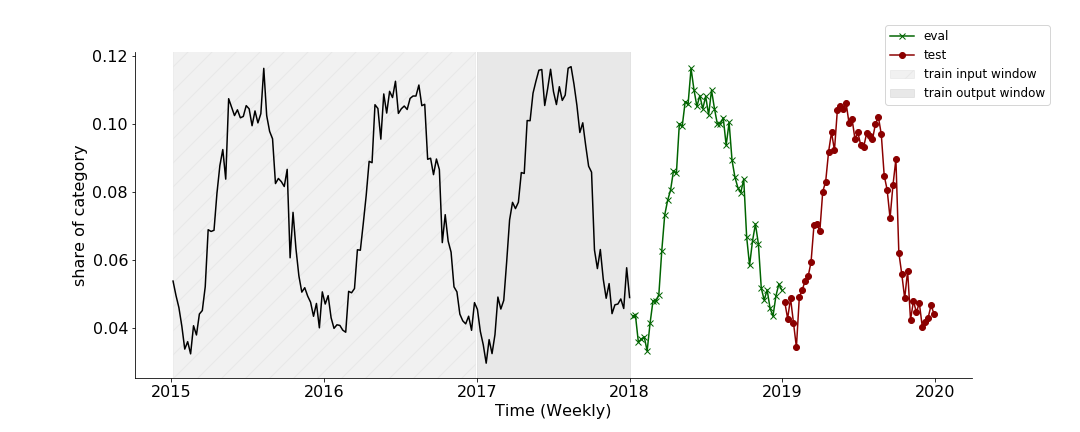
\includegraphics[width=1.\linewidth]{figure/train_eval_test_set}
  \caption{Temporal split for our training process. The three first years define our training set. The fourth year is used as our eval set and the final year is reserved for the test set.}
\label{fig:train_eval_test_set}
\end{figure*}

\begin{figure}
  \centering
    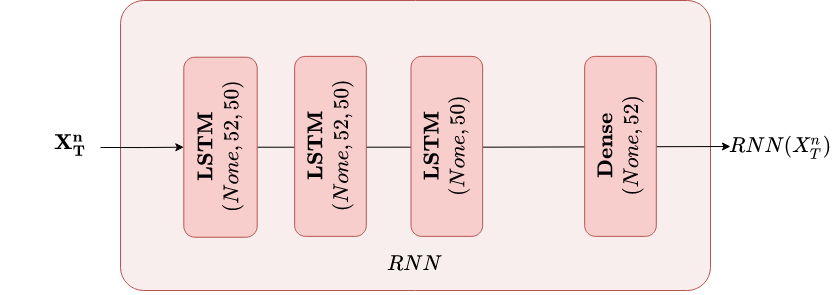
\includegraphics[width=0.8\linewidth]{figure/lstm_archi}
  \caption{Architecture of the RNN corrector part of the HERMES framework. The same architecture is used in the \textit{lstm} benchmark model.}
\label{fig:rnn_architecture}
\end{figure}

\subsection{Benchmarks, hybrid models and Metrics}

As benchmarks, several widespread statistical methods and deep learning approaches were selected. Using the R package \texttt{forecast} and the Python packages \texttt{statsmodels},  \texttt{tbats}, for each time series, predictions are computed with the following methods: \textit{snaive}, \textit{ets}, \textit{stlm}, \textit{thetam}, \textit{tbats} and \textit{auto.arima}. The forecast of the \textit{snaive} method is only the repetition of the last past period. The \textit{ets} model is an additive exponential smoothing with a level component and a seasonal component. The \textit{stlm} approach uses a multiplicative decomposition and models the seasonally adjusted time series with an exponential smoothing model. The \textit{Thetam} model decomposes the original signal in $\theta$-lines, predicts each one separately and recomposes them to produce the final forecast and \textit{tbats} uses a trigonometrical seasonality. Finally, \textit{auto.arima} is the R implementation of the ARIMA model with an automatic selection of the best parameters. A complete description and references for these models can be found in \cite{hyndman2020package}. As a deep learning approach, a full LSTM (\textit{lstm}) neural network composed of 3 LSTM layers of shape 50 and a final Dense layer of shape 52 is considered.
Two versions of HERMES are proposed. They are called respectively \textit{hermes-ets} and \textit{hermes-tbats} according to the per-time-series model choice. Moreover, two versions with the inclusion of the weak signals (ws) are proposed. They are referred to as \textit{hermes-ets-ws} and \textit{hermes-tbats-ws}. In order to provide a fair comparison, a \textit{lstm} with the weak signals named \textit{lstm-ws} is trained.

To compare the different methods, we use the Mean Absolute Scaled Error (MASE) for seasonal time series. As our sequences have completely different scales, from $10^{-5}$ to $10^{-1}$, this metric was chosen to compute a fair error measure, independent of the scale of the sequence and suited for our seasonal fashion time series. The MASE metric is defined as follows, with $m$ the seasonal period:
\begin{align*}
\mathrm{MASE} &= \frac{T-m}{h}\frac{\sum_{j=1}^h |Y_{T+j} - \hat{Y}_{T+j}| }{\sum_{i=1}^{T-m} |Y_i - Y_{i-m}|}\,.
\end{align*}
Detecting emerging and declining trends is a crucial issue for the fashion industry. A correct or incorrect prediction could lead to good returns or massive waste due to overstock or unsold clothes. In addition to the MASE accuracy metric, the different methods are also evaluated on a classification task and especially differences between methods using weak signals or not. In a given year, an increasing trend is defined as a trend that does more than 5\% of growth on average with respect to the previous year. In the same way, a decreasing trend is defined as a trend that declines by 5\% on average or more. Other trends are classified as flat trends. With this threshold, the proposed fashion dataset is almost balanced on the {\em test} set: There are 3087 increasing trends, 3342 decreasing trends and 3571 flat trends.
%On the {\em test} set, for each method, the accuracy is defined as follows:
%\begin{align*}
%\mathrm{ACCURACY} &= \frac{TP}{TP + FP}\,,
%\end{align*}
%where $TP = TP_{dec} + TP_{flat} + TP_{inc}$ and $FP = FP_{dec} + FP_{flat} + FP_{inc}$ with $TP_i$  the number of time series correctly classified in the class $i$ and $FP_i$ the number of time series misclassified in the class $i$.


\subsection{Result for Heuritech Fashion dataset}

\textbf{10000 Heuritech Fashion time series global accuracy. }For the two metrics and for each model, we compute the average on all sequences in the final year. Results are displayed in Table~\ref{tab:metricresults}. For our model using neural networks, 10 models are trained  with different seeds. The average and the standard deviation of their results are computed and displayed. For the statistical models, TBATS largely dominates the alternatives  in terms of MASE. It is one of the main motivations why this model is used on the best HERMES candidate as the predictor model. 

Considering the new HERMES approach, \textit{hermes-tbats} and \textit{hermes-tbats-ws} slightly outperform the alternatives in terms of MASE and are stable across the different trainings. Regarding \textit{hermes-ets},   although it is very similar to the baseline \cite{smyl2020hybrid}, its accuracy remains low in comparison to the \textit{lstm} benchmark or HERMES using TBATS. 

Models using our weak signals perform similarly as without-weak-signals models for the MASE.  Interestingly, weak signals significantly improve the accuracy in detecting emerging and declining trends. Figure~\ref{fig:examples} displays some examples of \textit{hermes-tbats} models and some weaknesses that can be corrected.

\begin{table}
  \caption{Results summary on the 10000ts Fashion dataset. For each metric, the average on all our time series is computed. For approaches using neural networks, 10 models are trained with different seeds. The mean and the standard deviation of the 10 results are displayed.}
  \centering
%  \resizebox{0.85\textwidth}{!}{%
  \begin{tabular}{l||lllll|lllll}
   &&\multicolumn{3}{c}{\textbf{MASE $\downarrow$}} &&& \multicolumn{3}{c}{\textbf{ACCURACY $\uparrow$}}&\\
    &&  \textit{mean}  && \textit{std} &&&  \textit{mean}  && \textit{std}& \\
%    \hline
	 \hline
	 &&&&&&&&&&\\
     \textit{snaive} && 0.881 && - &&& 0.357 && - &\\
     \textit{thetam}  && 0.844 && -&&& 0.482 && - &\\
     \textit{arima} && 0.826 && -&&& 0.464 && - & \\
     \textit{ets} && 0.807 && -&&& 0.449 && - & \\
     \textit{stlm} && 0.770 && -&&& 0.482 && - & \\
     \textit{hermes-ets-ws} && 0.769 && 0.005 &&& 0.501 && 0.007 &\\
     \textit{hermes-ets} && 0.758 && 0.001 &&& 0.490 && 0.006 &\\
     \textit{tbats} && 0.745 && -&&& 0.453 && - & \\
     \textit{lstm-ws} && 0.728 && 0.004 &&& 0.500 && 0.008 &\\
     \textit{lstm} && 0.724 && 0.003 &&& 0.498 && 0.007 &\\
     \textit{hermes-tbats} && 0.715 && 0.002 &&& 0.488 && 0.008 &\\
     \textbf{\textit{hermes-tbats-ws}} && \textbf{0.712} && 0.004 &&& \textbf{0.510} && 0.005 &\\
    %\hline
  \end{tabular}
%  }
\label{tab:metricresults}
\end{table}

\begin{figure*}
\centering
%\begin{subfigure}{1.\textwidth}
 % \centering
  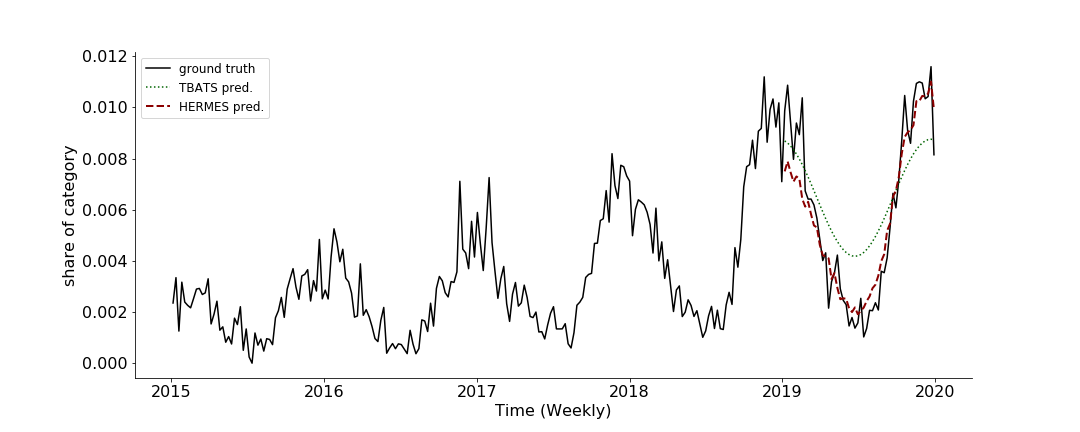
\includegraphics[width=1.\linewidth]{figure/us_female_top}
  %\caption{Time series representing a top fashion trend for female in The United States}
  %\label{fig:examples:sub1}
%\end{subfigure}
%\begin{subfigure}{1.\textwidth}
 % \centering
  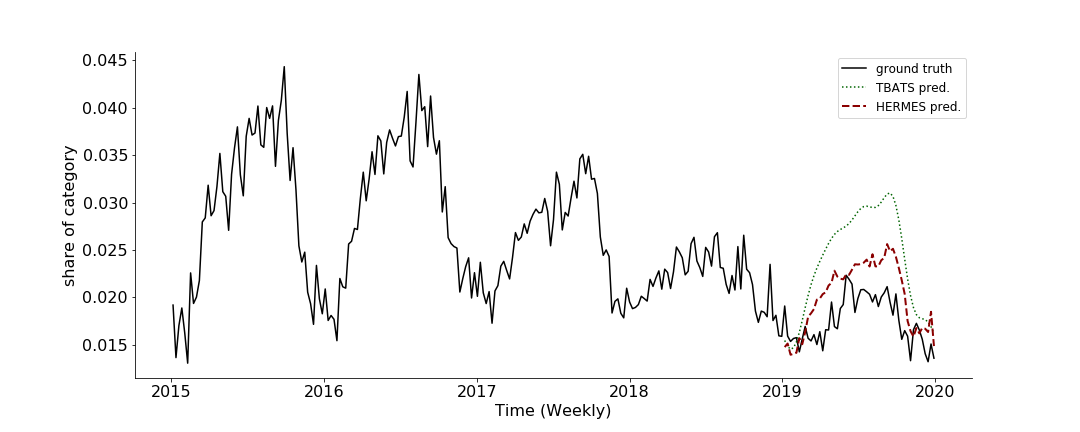
\includegraphics[width=1.\linewidth]{figure/cn_female_texture_horizontalstripe}
  %\caption{Time series representing the horizontal stipes texture fashion trend for female in China}
  %\label{fig:examples:sub2}
%\end{subfigure}
\caption{\textit{hermes-tbats} forecast examples. In green the prediction of the per-time-series predictors \textit{tbats}. In red the final forecast of our HERMES hybrid model \textit{hermes-tbats}. (Top) Time series representing a top fashion trend for females in The United States. (Bottom) Time series representing the horizontal stipes texture fashion trend for females in China.}
\label{fig:examples}
\end{figure*}

\textbf{10000 Heuritech Fashion time series classification task. } Classification results between the \textit{tbats} model and the hybrid method \textit{hermes-tbats} are given in Table~\ref{tab:tbatsclass}, we note an impressive decrease of impactful errors: i.e. forecasting an increase instead of a decrease and vice versa. The \textit{hermes-tbats} model divides by 3 the error rate in comparison to \textit{tbats} with only a slight decrease of the number of correct increase/decrease predictions. However, with our weak signals, we see that \textit{hermes-tbats-ws} is able to catch twice as much as its relative model without weak signals while keeping a relatively low number of impactful errors.

\begin{table}
  \caption{\textit{tbats}, \textit{hermes-tbats} and \textit{hermes-tbats-ws} models confusion matrix}
  %\vspace{0.2cm}
  %\textit{tbats} model confusion matrix \\
  %\par \textit{tbats} model confusion matrix
  %\vspace{0.2cm}
\centering
\vspace{0.2cm}
\resizebox{6cm}{!}{
  \begin{tabular}{l||llll}
  	&& \multicolumn{3}{c}{\textbf{\textit{tbats}}}\\
    && pred-dec  & pred-flat & pred-inc  \\
    \hline
    \hline
    \rule{0pt}{2ex} \\
	true-dec && 902 & 2113 & 327 \\
    true-flat && 351 & 2920 & 300 \\
    true-inc && 300 & 2078 & 709 
  \end{tabular}
}
\vspace{.2cm}
\resizebox{6cm}{!}{
  \begin{tabular}{l||llll}
  	&& \multicolumn{3}{c}{\textbf{\textit{hermes-tbats}}}\\
    && pred-dec  & pred-flat & pred-inc  \\
    \hline
    \hline
    \rule{0pt}{2ex} \\
	true-dec && 1261 & 1960 & 121 \\
    true-flat && 549 & 2823 & 199 \\
    true-inc && 214 & 2004 & 869 
  \end{tabular}
}
\vspace{.2cm}
\resizebox{6cm}{!}{
  \begin{tabular}{l||llll}
    && \multicolumn{3}{c}{\textbf{\textit{hermes-tbats-ws}}}\\
    && pred-dec  & pred-flat & pred-inc  \\
    \hline
    \hline
    \rule{0pt}{2ex} \\
	true-dec && 1956 & 1245 & 141 \\
    true-flat && 1257 & 2087 & 227 \\
    true-inc && 358 & 1620 & 1109 
  \end{tabular}
}
\label{tab:tbatsclass}
\end{table}

\textbf{Size of the dataset. } In addition to the results on the fashion dataset gathering 10000 time series, the behaviour of the HERMES model is analyzed when it is trained on smaller datasets: two experiments were performed, HERMES models were trained on a reduced dataset of 1000 time series and on a reduced dataset of 100 time series. Results are given in Table~\ref{tab:1000metricresults}.

First, the hybrid framework \textit{hermes-tbats} achieves the best performance in terms of global accuracy on both datasets. Due to the strength of its per-time-series predictor TBATS, the hybrid model succeeds at correcting TBATS  and reaches a satisfactory final accuracy. Secondly, we can note that the accuracy of the full neural network \textit{lstm} decreases when the dataset size decreases. On the small dataset of 100 time series, a local statistical model like \textit{tbats} or \textit{stlm} largely outperforms its accuracy level. Providing sharp predictions from scratch is a complex task and high-dimensional recurrent neural networks require  large amounts of data to do so. Nevertheless, with the HERMES framework, the RNN task is largely simplified. Our model needs less data to be trained and to obtain interesting performance.


\begin{table}
  \caption{Results summary on the 1000 time series and 100 time series Fashion dataset. The MASE average on all our time series is computed. For the two approaches using a neural network, 10 models with different seeds are trained. the mean and the standard deviation of the 10 results are displayed.}
 \centering
 \resizebox{1.\textwidth}{!}{ 
  \begin{tabular}{l||llll}
    \multicolumn{4}{c}{1000 time series Fashion dataset}\vspace{0.5cm} \\
    &&\multicolumn{2}{c}{\textbf{MASE}} \\
    &&  \textit{mean}  & \textit{std}  \\
%    \hline
	 \hline
	 &&& \\
     \textit{snaive} && 0.871 & - \\
     \textit{thetam}  && 0.849 & - \\
     \textit{arima} && 0.821 & - \\
     \textit{ets} && 0.801 & - \\
     \textit{stlm} && 0.765 & - \\
     \textit{lstm} && 0.740 & 0.007 \\
     \textit{tbats} && 0.734 & - \\
     \textbf{\textit{hermes-tbats}} && \textbf{0.719} & 0.002 \\
  \end{tabular}\hspace{1cm}
\vspace{.2cm}

  \begin{tabular}{l||llll}
   \multicolumn{4}{c}{100 ts Fashion dataset}\vspace{0.5cm} \\
   &&\multicolumn{2}{c}{\textbf{MASE}} \\
    &&  \textit{mean}  & \textit{std}  \\
%    \hline
	\hline
	 &&& \\
     \textit{snaive} && 0.876 & - \\
     \textit{thetam}  && 0.823 & - \\
     \textit{arima} && 0.814 & - \\
     \textit{ets} && 0.785 & - \\
     \textit{lstm} && 0.767 & 0.045 \\
     \textit{stlm} && 0.742 & - \\
     \textit{tbats} && 0.745 & - \\
     \textbf{\textit{hermes-tbats}} && \textbf{0.739} & 0.003 \\
  \end{tabular}
 }
\label{tab:1000metricresults}
\end{table}


\subsection{Result for M4 weekly dataset}

We also assessed the performance of HERMES using the M4 weekly dataset \cite{makridakis2020m4}. The M4 dataset gathers 359 weekly time series and has 3 main differences compared to our proposed fashion dataset. Firstly, sequences do not have the same length with sequence lengths lying between 93 and 2610 time steps. Secondly, as some of the sequences represent financial signals or some others are demographic sequences, the  359 time series have very distinct scales and dynamics. Thirdly, compared to the previous fashion application, the time horizon of the prediction is set to 13 for the weekly dataset. 

\textbf{Training. } The M4 dataset is firstly preprocessed. This preliminary step is motivated by two reasons. First, as some sequences are short (93 time steps), they limit the window size $w$ of the RNN part and consequently the global accuracy of the HERMES approach. Second, the longer time series slow down the training of the collection of the first predictors especially for complex methods like TBATS. We kept 300 time steps  for each sequence in order to train the HERMES model. For the shorter sequences, the train set is duplicated in order to reach the length of 300. Longer sequences are cropped in order to keep the last 300 time steps.
%The sequences are firstly resized in order to obatain a dataset with fixed time horizon. The eval and the test sets are removed for the shortest sequences (the last 26 steps). Then, the remaining number of entire year is duplicated in order to egalize all the sequence at the longest one : 2610 time steps \textcolor{red}{Pas sur de comprendre, reformuler}. As per time series parametric model training time depends on the sequence length, all time series are then croped. Finally, with the addition of the previously removed eval and test sets, 300 time steps are kept for each sequence \textcolor{red}{Pas sur de comprendre, reformuler}. 

The horizon $h$ is set to 13  and the window size $w$ is set to 104. For the RNN part, the same architecture as the one described in Figure~\ref{fig:rnn_architecture} is used. The Adam optimizer is used with a learning rate  equal to  0.005 and a batch size set to 8. As the M4 weekly dataset is small, a rolling window is used on the train set in order to increase the train number of examples and improve training results. Three windows are computed for each sequence for the RNN train set. An overview of our train, eval, test set split and the resizing of the shortest sequences is given in Figure~\ref{fig:m4dataset}.
The previous parameters: window size, learning rate, batch size and the number of train windows per time series are set using a grid search, see Appendix~B.

\begin{figure*}
  \centering
    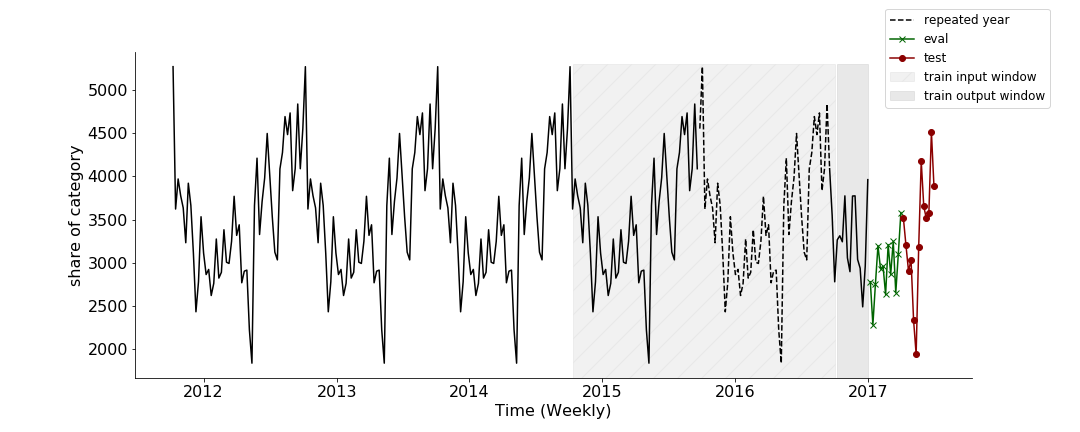
\includegraphics[width=1.\linewidth]{figure/M4_dataset}
  \caption{One of the shortest sequences of the M4 weekly dataset (93 time steps). In order to fit its predictor, the last complete year is duplicated in order to reach a total length of 300 time steps.}
\label{fig:m4dataset}
\end{figure*}

\textbf{Benchmarks. } The M4 competition provides a rich collection of benchmarks emcompassing statistical models and neural network approaches. The same candidates are used in this part as baselines. In addition, the hybrid model named \textit{Uber} of S.Smyl is added. For a complete description and references of the benchmark models, see \cite{makridakis2020m4}. As a HERMES candidate, a version using TBATS is proposed and called \textit{hermes-tbats}. Following the M4 competition methodology, models are evaluated according to the MASE, the SMAPE and the OWA measures. A complete definition of these metrics is proposed in \cite{makridakis2020m4}, see also Appendix~\ref{sec:m4overview} for additional information about the M4 weekly dataset.

\textbf{Results and discussion. } The final results for the M4 weekly dataset are displayed in Table~\ref{tab:m4metricresults}. The HERMES approach \textit{hermes-tbats} outperforms all the benchmarks. This result is partially induced by the use of TBATS per-time-series predictors which achieves very good results on the test set. Regarding the hybrid model proposed by S.Smyl, its accuracy remains low in comparison to \textit{tbats} and  \textit{hermes-tbats}. With this second application, two important conclusions can be made. Firstly, the results provided by \textit{hermes-tbats} confirm that the HERMES approach is a general framework, well suited for a large collection of forecasting tasks. Secondly, the accuracy gap between the two hybrid candidates validates the HERMES approach and illustrates the importance of a global framework able to leverage any kind of per-time-series predictors.

\begin{table*}
  \caption{Results summary on the m4 weekly dataset. For each metric, the average on all our time series is computed. For approaches using a neural network, 10 models are trained with different seeds. The mean and the standard deviation of the 10 results are displayed.}
  \centering
  \resizebox{\textwidth}{!}{
  \begin{tabular}{l||lllll|lllll|lllll}
   &&\multicolumn{3}{c}{\textbf{SMAPE}} &&& \multicolumn{3}{c}{\textbf{MASE}} &&& \multicolumn{3}{c}{\textbf{OWA}}&\\
    &&  \textit{mean}  && \textit{std} &&&  \textit{mean}  && \textit{std}&&&  \textit{mean}  && \textit{std}& \\
%    \hline
	 \hline
	 &&&&&&&&&&\\
     \textit{MLP} && 21.349 && - &&& 13.568 && - &&& 3.608 && - &\\
     \textit{RNN} && 15.220 && - &&& 5.132 && - &&& 1.755 && - &\\
     \textit{snaive} && 9.161 && - &&& 2.777 && - &&& 1.000 && - &\\
     \textit{SES} && 9.012 && - &&& 2.685 && - &&& 0.975 && - &\\
     \textit{Theta} && 9.093 && - &&& 2.637 && - &&& 0.971 && - &\\
     \textit{Holt} && 9.708 && - &&& 2.420 && - &&& 0.966 && - &\\
     \textit{Com} && 8.944 && - &&& 2.432 && - &&& 0.926 && - &\\
     \textit{Damped} && 8.866 && - &&& 2.404 && - &&& 0.917 && - &\\
     \textit{S.Smyl} \cite{hyndman2020package} && 7.817 && - &&& 2.356 && - &&& 0.851 && - &\\
     \textit{tbats} && 8.111 && - &&& 2.214 && - &&& 0.841 && - &\\
     \textit{\textbf{hermes-tbats}} && \textbf{7.597} && 0.113 &&& \textbf{2.205} && 0.042 &&& \textbf{0.812} && 0.011 &\\
    %\hline
  \end{tabular}
  }
\label{tab:m4metricresults}
\end{table*}


\section{Conclusion}
\label{sec:conclusion}
The motivation of this paper was to present HERMES, a new hybird model for non stationary time series forecasting. By mixing the performance of local parametric models and a global neural network, \textit{hermes-tbats} clearly outperforms traditional statistical methods and full neural network models on two forecasting tasks. Furthermore, this new model is totally suited to deal with external signals. With a fine pre-processing and a well-designed architecture, our hybrid framework succeeds at leveraging our complex extra data and reaches very promising accuracy levels in terms of classification. In addition to this article, a fashion dataset gathering a sample of $\numberts$ time series and a collection of weak signals is provided. We believe that this dataset contains really fine dynamics and interactions where complex models would express their potential. By making it publicly available\footnote[1]{\url{http://files.heuritech.com/raw_files/f1_fashion_dataset.tar.xz}}, we hope that it will enhance the diversity of datasets for time series forecasting and pave the way for further explorations.
As a possible future work, designing new models for the weak signals would improve their inclusion  in the HERMES architecture. Focusing on the examples with huge changes of behaviours, a fine analysis of the impact of the collection of weak signals is the topic of ongoing works. In the same way, an interesting improvement of the hybrid framework can be to introduce not a single but several neural networks trained at correcting different kinds of weaknesses. A perspective is to add a latent discrete label to select dynamically the regime shifts. 


%\appendices

%\renewcommand{\thetable}{A\arabic{table}}
%\renewcommand{\thefigure}{A\arabic{figure}}
%\setcounter{table}{0}
%\setcounter{figure}{0}


\section*{Appendix A. M4 weekly dataset and results}
\label{sec:m4overview}


The M4 weekly dataset is a collection of 359 time series with  contrasting behaviours and sizes. An overview of the dataset is given in Table~\ref{tab:m4dataset} and some examples of sequences are given in Figure~\ref{fig:m4examples}. As sequences come from a wide diversity of sectors, the forecasting task is very challenging. However, on some examples as in Figure~\ref{fig:m4pred}, efficient corrections of the TBATS forecasts can be obtained.

\begin{table}

  \caption{M4 weekly dataset overview. For each category, the number of sequences and the average length are given.}
\label{tab:m4dataset}
  \centering
  \resizebox{0.8\width}{!}{
  \begin{tabular}{l||lll}
    %hline
    \\
    &  \textbf{Nb. of sequences}  & \textbf{Avg. length} & \textbf{Min. length} \\
    \hline
    \hline
    \\
	\textbf{Demographic} & 24 & 1659 & 1615\\
	\textbf{Finance} & 164 & 1237 & 260\\
	\textbf{Industry} & 6 & 834 & 356\\
	\textbf{Macro} & 41 & 1264 & 522\\
	\textbf{Micro} & 112 & 473 & \textbf{93}\\
	\textbf{Other} & 12 & 1598 & 470\\
  \end{tabular}
  }
\end{table}


\begin{figure}
%\centering
%\begin{subfigure}{.45\textwidth}
%  \centering
  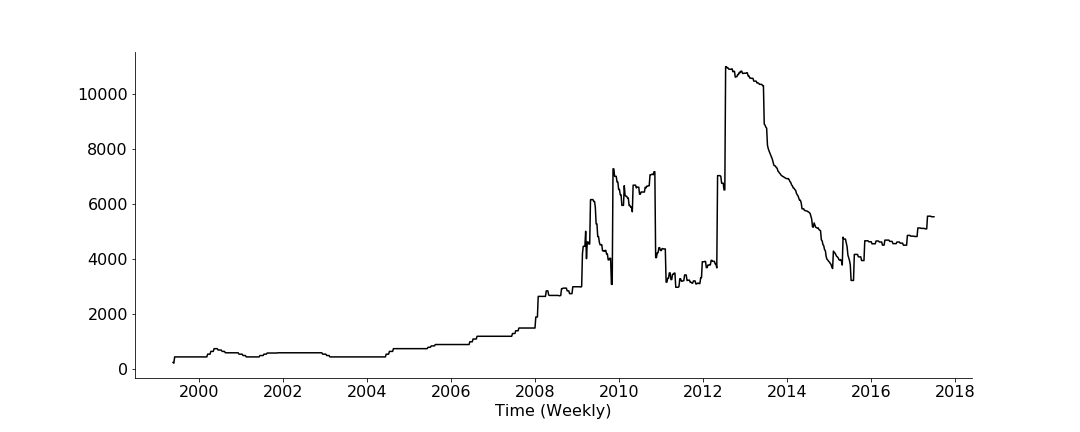
\includegraphics[width=1.\linewidth]{figure/W10}
%  \caption{A time series from the ``Other`` category called \textit{W10}.}
  \label{fig:m4examples:sub1}
%\end{subfigure} \quad
%\begin{subfigure}{.45\textwidth}
%  \centering
  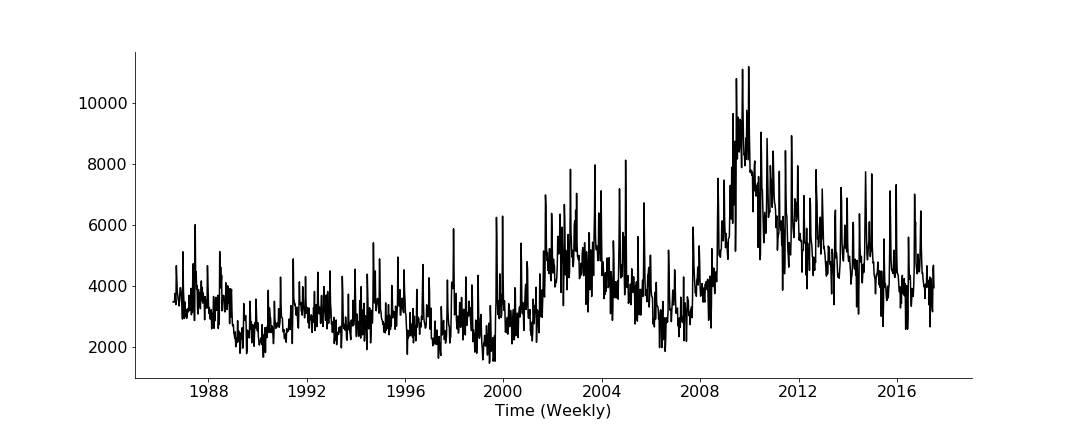
\includegraphics[width=1.\linewidth]{figure/W20}
%  \caption{A time series from the ``Macro`` category called \textit{W20}.}
%  \label{fig:m4examples:sub1}
%\end{subfigure}
%\begin{subfigure}{.45\textwidth}
%  \centering
  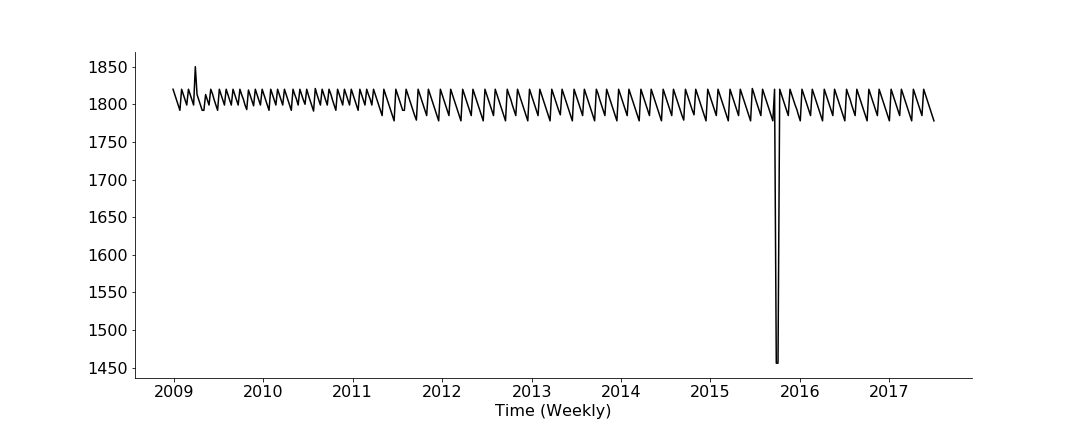
\includegraphics[width=1.\linewidth]{figure/W220}
%  \caption{A time series from the \textit{Finance} category called \textit{W220}.}
%  \label{fig:m4examples:sub2}
%\end{subfigure}\quad
%\begin{subfigure}{.45\textwidth}
%  \centering
%  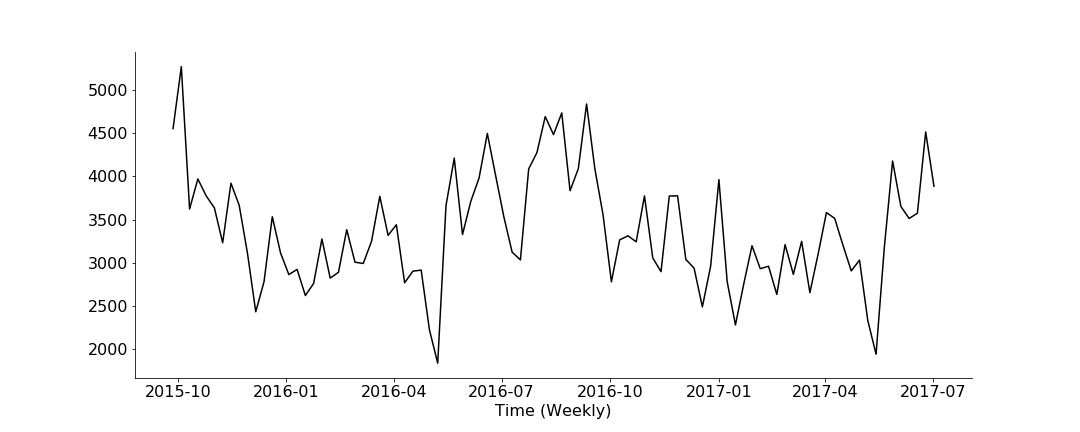
\includegraphics[width=1.\linewidth]{figure/W354}
%  \caption{A time series from the \textit{Micro} category called \textit{W354}.}
%  \label{fig:m4examples:sub3}
%\end{subfigure}
\caption{Examples of time series from the M4 weekly dataset. From Top to Bottom : time series called \textit{W10} from the \textit{Other} category, \textit{W20} from the \textit{Macro} category and \textit{W220} from the \textit{Finance} category.}
\label{fig:m4examples}
\end{figure}

\begin{figure*}
\centering
% \begin{subfigure}{1.\textwidth}
%  \centering
  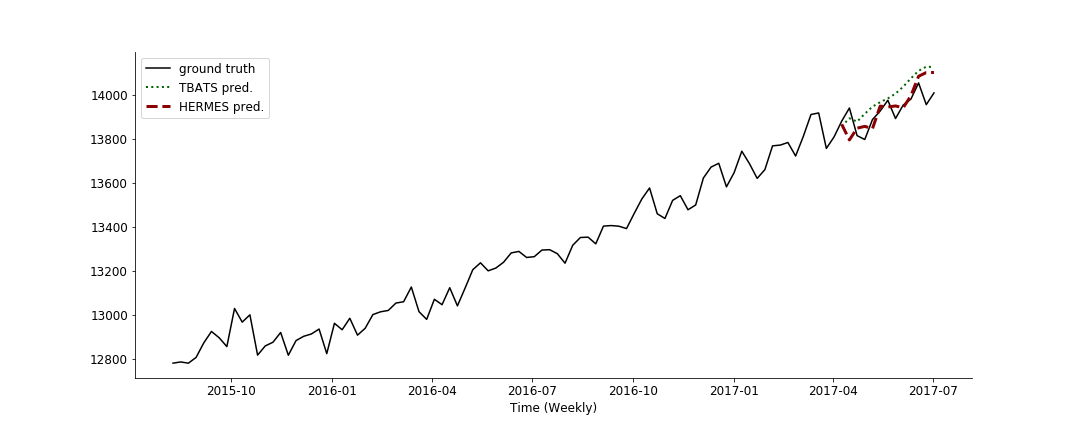
\includegraphics[width=1.\linewidth]{figure/W133_pred}
%  \caption{\textit{tbats} and \textit{hermes-tbats} forecast of the \textit{W133} time series}
%  \label{fig:m4pred:sub1}
% \end{subfigure}
% \begin{subfigure}{1.\textwidth}
%  \centering
  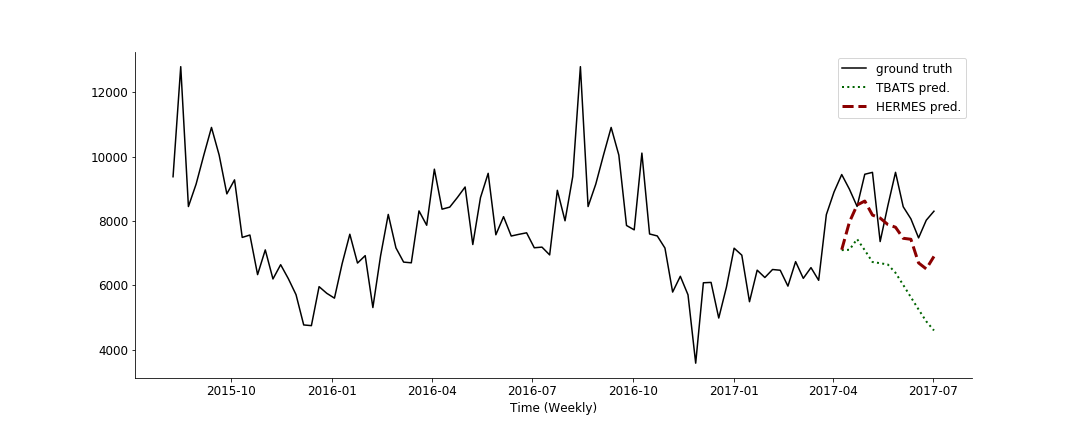
\includegraphics[width=1.\linewidth]{figure/W314_pred}
%  \caption{\textit{tbats} and \textit{hermes-tbats} forecast of the \textit{W314} time series}
%  \label{fig:m4pred:sub2}
% \end{subfigure}
\caption{\textit{hermes-tbats} forecast examples on the M4 weekly dataset. In green the prediction of the per-time-series predictors \textit{tbats}. In red the final forecast of our HERMES hybrid model \textit{hermes-tbats}. (Top) the \textit{W133} time series, (Bottom) the \textit{W314} time series.}
\label{fig:m4pred}
\end{figure*}


%Looking at the final result of the M4 competition, some models reach a higher accuracy than the HERMES framework on the weekly dataset. Except one approach, all of them are a combination of different models in order to increase the robustness of the final forecast and at the same time achieve a better global accuracy. The remaining one is not an ensembling but a statistical framework called \textit{Forecast Pro}. It is not a single statistical model but a framework that chooses, depending on the sequence properties, the best statistical approach. With a OWA equal to 0.739, it outperforms the \textit{hermer-tbats} and all the M4 proposed models on the M4 weekly sub-dataset. A description and interesting remarks about the \textit{Forecast Pro} model are discussed in \cite{DARIN2020135}. This model offers an interesting research perspective specifically for the M4 weekly forecasting task.
Looking at the final results of the M4 competition, some models reach a higher accuracy than the HERMES framework on the weekly dataset. All of them are ensemble frameworks: methods that mix different kinds of approaches to reach a higher final accuracy. As the M4 weekly dataset gathers really heterogeneous sequences, combining several methods to leverage their strengths appear to be a promising way. However in this paper, only individual models were evaluated in order to provide a fair comparison with the HERMES framework.

\section*{Appendix B. Training parameters and loss}


\subsection{Loss grid search on the Fashion Dataset}
\label{sec:heuritechgridsearch}

Using deep learning models in time series forecasting is an appealing way to achieve higher accuracy performance. However, it induces two main issues. First, it requires a large enough dataset to train the model as illustrated in Section~\ref{sec:exp}. Second, a dataset can hide contrasting time series in terms of scale, noise and behaviour. These differences can impact training performance. For the HERMES architecture, some candidate losses were defined for the training: the Mean Absolute Error (MAE), the Mean Square Error (MSE),  the Scaled Mean Absolute Error (SMAE) and the Scaled Mean Square Error (SMSE). The loss functions are defined as follows:
\begin{align*}
MAE &= \frac{1}{\lag}\sum_{i=1}^{\lag}|\ts^n_{T+i} - \tspred^n_{T+i|T}|\,,\\
MSE &= \frac{1}{\lag}\sum_{i=1}^{\lag}(\ts^n_{T+i} - \tspred^n_{T+i|T})^2\,,\\
SMAE &= \frac{1}{\meants^n_T}\sum_{i=1}^{\lag}|\ts^n_{T+i} - \tspred^n_{T+i|T}|\,,\\
SMSE &= \frac{1}{\meants^n_T}\sum_{i=1}^{\lag}(\ts^n_{T+i} - \tspred^n_{T+i|T})^2\,.
\end{align*}
For each loss, 10 \textit{hermes-tbats-ws} models have been trained with different seeds and the final mean and standard deviation are given in Figure~\ref{fig:loss_function}. The final Scaled Mean Absolute Error reaches the lowest MASE and was selected to train all the HERMES model in this paper.

\begin{figure}
  \centering
    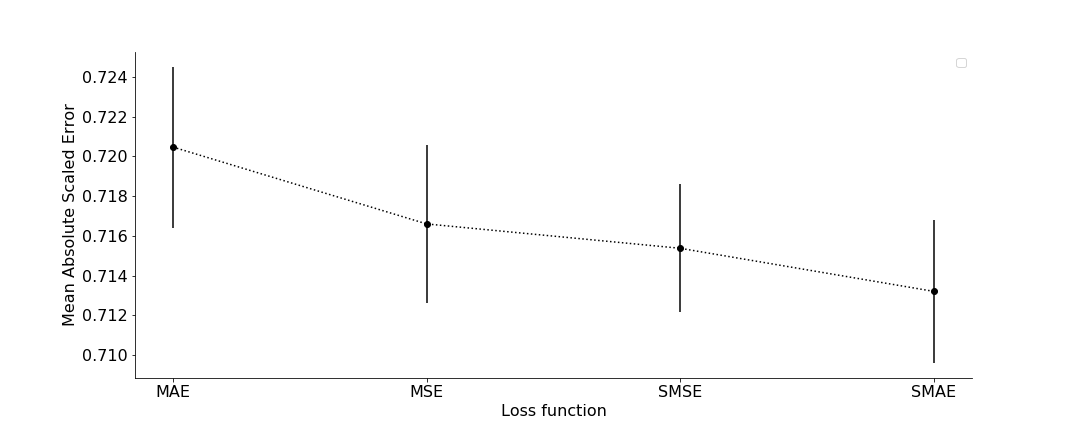
\includegraphics[width=1.\linewidth]{figure/loss_function}
  \caption{MASE accuray for the \textit{hermes-tbats-ws} model depending on the loss used during the RNN training. For each loss, 10 models with different seeds have been trained. The mean and the standard deviation are represented with a point and a vertical line.}
\label{fig:loss_function}
\end{figure}



\subsection{Parameters grid search on the M4 weekly Dataset}
\label{sec:m4gridsearch}

In addition to the loss function, the HERMES model also depends on several hyperparameters to set correctly in order to reach satisfactory performance. For instance, an overview of the learning rate, batch size and number of windows per time series grid search for the M4 weekly dataset is shown in Figure~\ref{fig:m4parameter}. For each parameter, a collection of 10 \textit{hermes-tbats} models have been trained with a range of values and the final OWA was calculated. As in the Figure~\ref{fig:loss_function}, the mean and the standard deviation of each group of 10 trainings is computed. For the final \textit{hermes-tbats} model of the M4 weekly dataset,  the following set of parameters was selected: 3 windows per time series were used as the train set, the batch size was set to 8 and the learning rate was fixed to 0.005.

 
\begin{figure}
\centering
%\begin{subfigure}{1.\textwidth}
 % \centering
  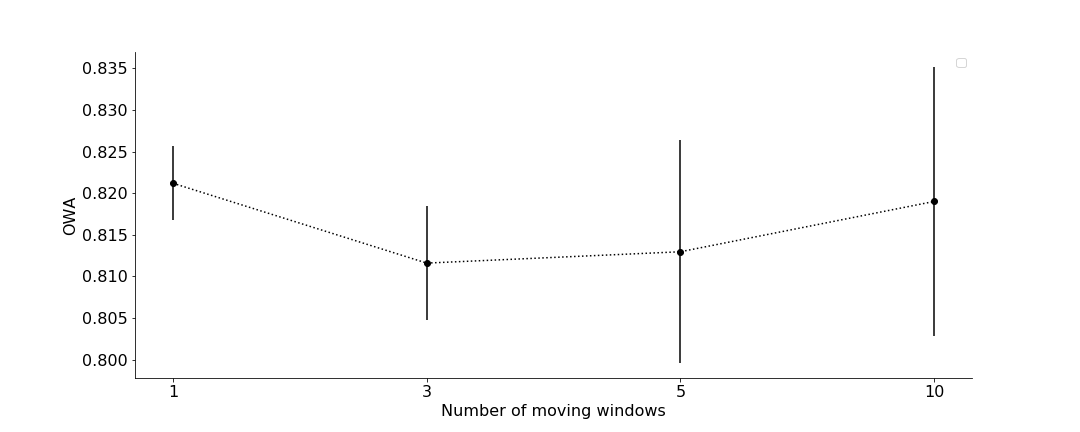
\includegraphics[width=1.\linewidth]{figure/m4_nb_of_window}
  %\caption{result of the HERMES model on the M4 dataset model depending of the number of windows provided per time series to the RNN corrector}
 % \label{fig:m4parameter:sub1}
%\end{subfigure}
%\begin{subfigure}{1.\textwidth}
 % \centering
  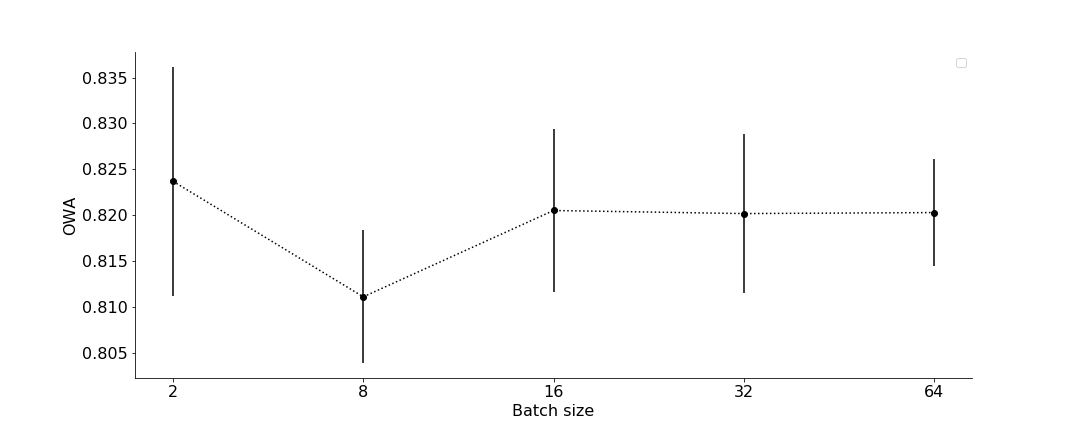
\includegraphics[width=1.\linewidth]{figure/m4_batch_size}
  %\caption{result of the HERMES model on the M4 dataset model depending of the size of the batch size}
  %\label{fig:m4parameter:sub2}
%\end{subfigure}
%\begin{subfigure}{1.\textwidth}
  %\centering
  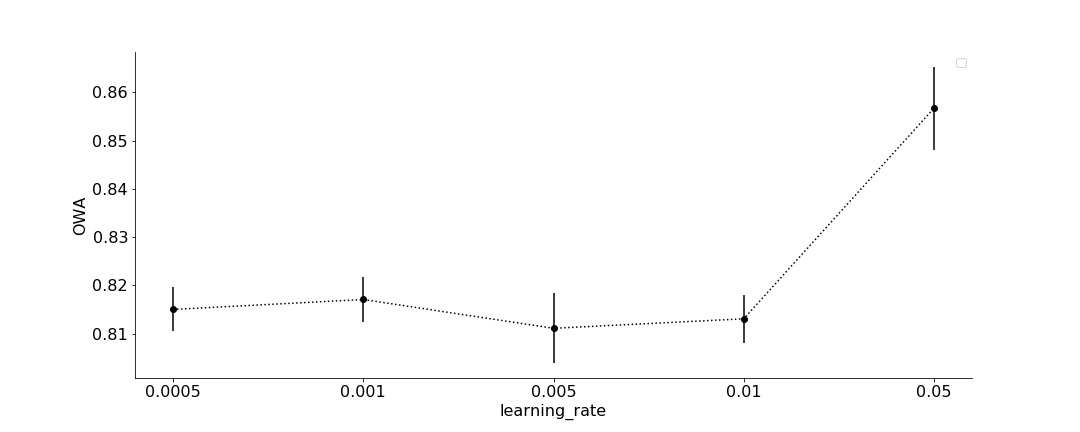
\includegraphics[width=1.\linewidth]{figure/m4_learning_rate}
  %\caption{result of the HERMES model on the M4 dataset model depending of learning rate of the optimizer}
  %\label{fig:m4parameter:sub3}
%\end{subfigure}
\caption{OWA for the \textit{hermes-tbats} model on the M4 weekly dataset depending on 3 parameters used during the RNN training: Number of moving windows per time series, the batch size and the learning rate. For each parameter, 10 models with different seeds have been trained. The mean and the standard deviation are represented with a point and a vertical. (Top) Result of the HERMES model depending on the number of windows provided per time series to the RNN corrector. (Middle) Result of the HERMES model depending on the size of the batch size. (Bottom) Result of the HERMES model depending on the learning rate of the optimizer.}
\label{fig:m4parameter}
\end{figure}

\section*{References}

\bibliography{hermes_paper_elsevier}

\end{document}